\documentclass[8pt,leqno,xcolor={dvipsnames,table},aspectratio=169]{beamer}

\IfFileExists{fontawesome.sty}{\usepackage{fontawesome}}{}
\usepackage{appendixnumberbeamer}
\newenvironment{fullframe}
{
\setbeamertemplate{background}{}%
\begin{frame}[plain,t]%
}
{
\end{frame}%
}
\newenvironment{fullpage}{%
  \begin{list}{}{%
    \setlength{\topsep}{0pt}%
    \setlength{\leftmargin}{-1cm}%
    \setlength{\rightmargin}{-1cm}%
    \setlength{\listparindent}{\parindent}%
    \setlength{\itemindent}{\parindent}%
    \setlength{\parsep}{\parskip}%
  }%
\item[]
\vspace{-7\lineskip}}
{\end{list}}

\graphicspath{{./img/}{./images/}}

\usepackage{graphicx, color}
\definecolor{xpol}{RGB}{1,66,106}%{0.086,0.141,0.164}
\definecolor{adia}{RGB}{1,66,106}%{0.086,0.141,0.164}
\definecolor{liwa}{RGB}{184,206,224}
\definecolor{adiared}{RGB}{224,167,110}%{0.086,0.141,0.164}
\usepackage{pifont}

\usetheme[%
progressbar=head,titleformat=regular,numbering=fraction,subsectionpage=progressbar%
]{metropolis} % sectionpage=progressbar
\usecolortheme{seahorse}
\usepackage[T1]{fontenc}
\usepackage{concrete}
\setbeamercolor{progress bar}{fg=adia}
\setbeamercolor{frametitle}{fg=adia,bg=adia!20}
\makeatletter
\setlength{\metropolis@titleseparator@linewidth}{2pt}
\setlength{\metropolis@progressonsectionpage@linewidth}{2pt}
\setlength{\metropolis@progressinheadfoot@linewidth}{2pt}
\makeatother
\makeatletter
\addtobeamertemplate{sidebar right}{}{%
  \begin{tikzpicture}[remember picture,overlay] %
    \node[anchor=south east,xshift=0pt,yshift=0pt,opacity=0.4] at (current page.south east) {\includegraphics[width=0.2\paperwidth]{cmap-margin-low.png}};% x_progress
  \end{tikzpicture} }
\makeatother

\AtBeginSection{
  \frame{
    \sectionpage
    \tableofcontents[currentsection,hideallsubsections]
  }
  \addtocounter{framenumber}{-1}
}

\usepackage[listings,theorems]{tcolorbox}
\newenvironment{squaredblock}[2]{%
\begin{tcolorbox}[colback=adia!15,colframe=adia!85!black,title={#1}]% 
#2}{\end{tcolorbox}}

\usepackage{booktabs}
\usepackage{amsmath,amssymb}

\def\polbf#1{{\color{adia}{\bf #1}}}
\def\polbox#1{\colorbox{adia!15}{{\color{adia!85}\bf #1}}}
\setbeamercolor{button}{bg=black!35,fg=white}
\def\pollink#1#2{\hyperlink{#1}{\beamergotobutton{#2}}}
\setbeamercolor{alerted text}{fg=adia}
\def\wpolbox#1#2{\adiabox{\rule{#1}{0pt}#2 \rule{#1}{0pt}}}
\def\polbutton#1#2{\hyperlink{#1}{\beamergotobutton{#2}}}

\let\cfmbf=\adiabf
\let\cfmbox=\adiabox
\def\tightlist{}

\def\xipptitlelogo{%
  \includegraphics[width=.75\linewidth]{logo_polytechnique_ipp.pdf}
}

\setbeamertemplate{frame footer}{C.-A. Lehalle}
\author[C.A. Lehalle]{}
\institute[{CMAP, Ecole Polytechnique}]{}

\title{Clustering, Prototype Narratives, and Stiefel-Manifold Orthogonalization:}
\subtitle{A Worked Methodology on CNN Live-Blog Coverage of the 2026 Iran War}
\date{ \normalsize {\color{xpol}\bf Charles-Albert Lehalle}\hfill {\includegraphics[width=.08\linewidth]{logo_polytechnique_ipp.pdf}}\\[.3em]%
  \small CMAP, Ecole Polytechnique, IP Paris\\[.3em]%
  \small Following the Anglade-Lehalle-Massi approach of orthogonalisation of narratives\\[.3em]%
  \small Printed the Aug 21, 2026}

\usepackage{bbm}
\def\bm#1{\mathbf{#1}}
\newcommand*\circled[1]{\tikz[baseline=(char.base)]{
    \node[shape=circle,draw,inner sep=2pt] (char) {#1};}}
\newcommand*\bfcircled[1]{\tikz[baseline=(char.base)]{
    \node[shape=circle,draw,inner sep=2pt, fill=adia!15, line width=1.5pt, draw=adia] (char) {\polbf{#1}};}}

\def\R{\mathbbm{R}}
\def\Esp{\mathbb{E}}
\def\one{\mathbf{1}}
\def\softmax{\text{\sf softmax}}
\def\Id{\textbf{\sf Id}}
\def\Pr{\mathbb{P}}
\def\calD{{\cal D}}
\def\calV{{\cal V}}

\let\toprule=\hline
\let\midrule=\hline
\let\bottomrule=\hline
\let\mybox=\adiabox 
\let\mybf=\adiabf

\begin{document}

\begin{frame}[plain]
  \titlepage 
\end{frame}

\begin{frame}
  \frametitle{Positioning: What Are We Talking About?}

  \begin{squaredblock}{The problem}
  A corpus of \polbf{1{,}572} paragraph-level snippets from CNN's live-blog
  coverage of the US--Israel--Iran conflict (March--August 2026). We want to:
  \begin{itemize}
    \item discover the \polbf{narrative themes} present in the corpus,
    \item build a \polbf{clean, discriminative vector} representing each theme,
    \item and track any document's \polbf{exposure} to a theme over time --
      without that exposure being contaminated by generic ``war-reporting English''.
  \end{itemize}
  \end{squaredblock}

  \vspace{1em}
  \begin{squaredblock}{The idea, in one sentence}
  Cluster in the natural embedding space, build a short hand-written
  \polbf{prototype} per cluster, then \polbf{orthogonalize} the prototypes
  on the Stiefel manifold to strip out what all themes share, leaving a
  \polbf{pure narrative} per theme.
  \end{squaredblock}
\end{frame}

\begin{frame}
  \frametitle{Time to Conclude, Read Ahead: The Take-Away}
  \tableofcontents
\end{frame}
\addtocounter{framenumber}{-1}

% =========================================================================
\section{Overview of the Pipeline}
% =========================================================================

\begin{frame}
  \frametitle{Five Stages, From Raw Text to Validated Pure Narratives}

  \begin{enumerate}[leftmargin=1.4cm]
    \item[\bfcircled{1}] \polbf{Embed \& cluster} the corpus in its natural,
      untouched embedding space ($K=8$ clusters, K-Means on PCA scores).
    \item[\bfcircled{2}] \polbf{Curate \& average} three representative
      narratives per cluster into one \polbf{prototype of narrative}.
    \item[\bfcircled{3}] \polbf{Orthogonalize} the eight prototypes on the
      Stiefel manifold $\to$ \polbf{pure narratives}, purged of shared
      background noise.
    \item[\bfcircled{4}] \polbf{Score} every snippet against three
      representations: original / pure (orthogonal) / residual.
    \item[\bfcircled{5}] \polbf{Validate ex post}: does the pure
      representation separate in-cluster from out-of-cluster documents
      \emph{better} than the raw one?
  \end{enumerate}

  \vspace{1em}
  \begin{alertblock}{Why this matters}
  If pure narratives cleanly separate documents, then tracking a document's
  cosine similarity to a pure narrative \emph{over time} reflects genuine
  shifts in \polbf{exposure to that narrative} -- not drift in how much
  generic conflict vocabulary a day's reporting happens to use.
  \end{alertblock}
\end{frame}

% =========================================================================
\section{Stage 1: Embedding \& Clustering}
% =========================================================================

\begin{frame}
  \frametitle{Embedding and Clustering in the Natural Space}

  \begin{columns}[T]
    \begin{column}{0.48\textwidth}
      \begin{itemize}
        \item $n=1{,}572$ snippets, March 1 -- August 18, 2026
        \item Each snippet $\to$ unit-norm $\mathbf{e}_i \in \R^{768}$
          (\texttt{nomic-ai/modernbert-embed-base})
        \item $\text{sim}(s_i,s_j) = \mathbf{e}_i^\top \mathbf{e}_j$
        \item PCA to 50 dims (numerical stability only)
        \item K-Means, $K=8$, fit on the PCA scores
      \end{itemize}
      \vspace{.5em}
      \begin{alertblock}{Key methodological point}
      No orthogonalization or transformation is applied before or during
      clustering: whatever structure K-Means finds is a property of the
      embedding model and the corpus alone, not an artifact of the machinery
      introduced later.
      \end{alertblock}
    \end{column}
    \begin{column}{0.48\textwidth}
      \centering
      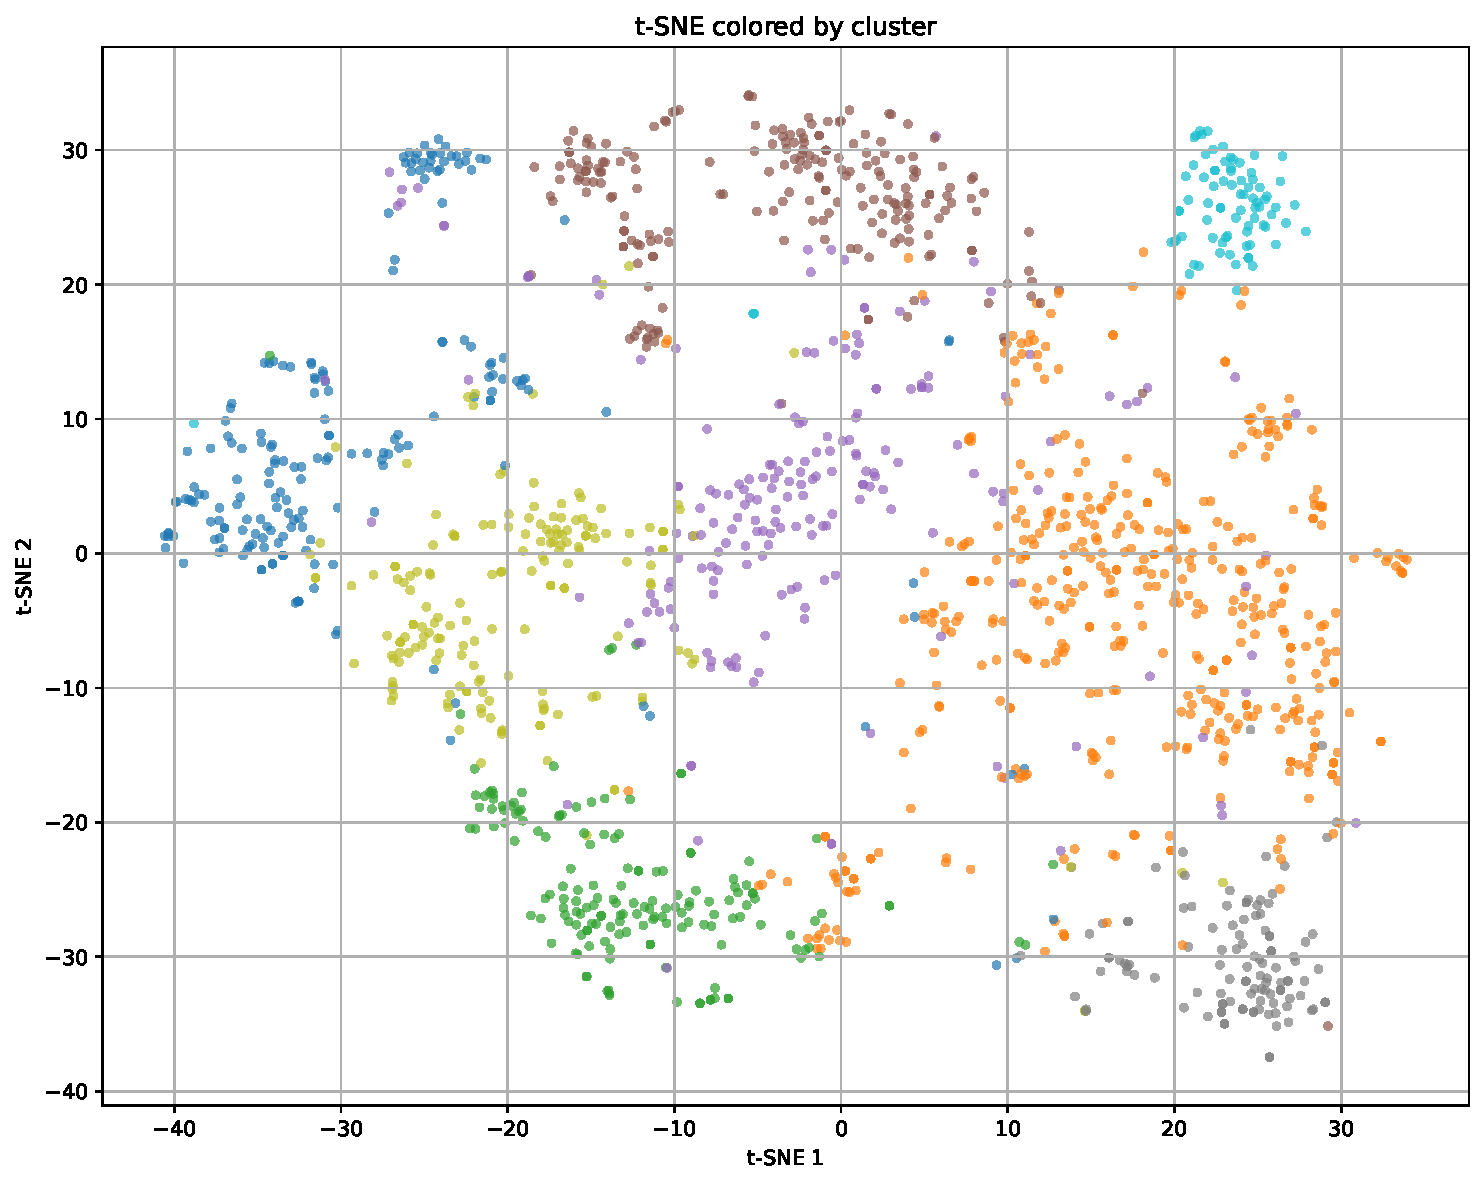
\includegraphics[width=\linewidth]{clusters_CNN.pdf}\\
      {\scriptsize t-SNE projection (diagnostic only), colored by K-Means cluster.}
    \end{column}
  \end{columns}
\end{frame}

\begin{frame}
  \frametitle{The Eight Clusters}

  \begin{center}
  \renewcommand{\arraystretch}{1.15}
  \begin{tabular}{clr}
    \toprule
    \bf \# & \bf Theme & \bf Size \\
    \midrule
    0 & Gulf Regional Military Escalation & 209 \\
    1 & Global Energy Markets \& Economic Fallout & 81 \\
    2 & Iranian Political Transition \& Internal Affairs & 110 \\
    3 & US-Israel Military Campaign in Iran & 246 \\
    4 & US Domestic Politics \& Presidential Leadership & 306 \\
    5 & Israel-Hezbollah-Lebanon Theater & 170 \\
    6 & Diplomacy \& International Mediation & 235 \\
    7 & \polbf{Maritime Conflict \& Strait of Hormuz} & 215 \\
    \midrule
    & \bf Total & \bf 1{,}572 \\
    \bottomrule
  \end{tabular}
  \end{center}

  \vspace{.5em}
  \small
  Worked example used throughout: \polbf{Maritime Conflict \& Strait of
  Hormuz} -- shipping disruption, tanker attacks, naval blockades, transit
  through the Strait.
\end{frame}

% =========================================================================
\section{Stage 2: Representative Narratives \& Prototypes}
% =========================================================================

\begin{frame}
  \frametitle{From Representative Narratives to a Prototype}

  \begin{squaredblock}{Worked example -- Maritime Conflict \& Strait of Hormuz}
  \small
  \begin{itemize}
    \item $r_{7,1}$: Maritime traffic through the Strait of Hormuz has
      slowed to a near halt as shipping companies reroute or suspend passage.
    \item $r_{7,2}$: US forces intercepted and seized a cargo vessel
      attempting to bypass the naval blockade of Iranian ports.
    \item $r_{7,3}$: An oil tanker was struck and disabled by an
      unidentified projectile near the strait's entrance.
  \end{itemize}
  \end{squaredblock}

  \vspace{1em}
  Three hand-picked, illustrative sentences per cluster (curated by the
  analyst, \emph{not} the medoid/centroid), embedded and averaged:
  \[
  N_i = \frac{\frac{1}{3}\sum_{k=1}^3 r_{i,k}}{\left\lVert \frac{1}{3}\sum_{k=1}^3 r_{i,k}\right\rVert}, \qquad i=1,\dots,8
  \]

  \begin{itemize}
    \item Encodes the analyst's semantic understanding of the theme,
      independently of how K-Means partitioned the data.
    \item Averaging cancels idiosyncratic wording, keeps the common direction.
  \end{itemize}
\end{frame}

% =========================================================================
\section{Stage 3: Stiefel-Manifold Orthogonalization}
% =========================================================================

\begin{frame}
  \frametitle{The Problem: Prototypes Are Highly Correlated}

  \begin{columns}[T]
    \begin{column}{0.55\textwidth}
      \begin{itemize}
        \item Pairwise cosine similarity between the 8 prototypes: typically
          \polbf{0.6 -- 0.8} off-diagonal.
        \item Interpretation: a shared \polbf{background noise} --
        \begin{itemize}
          \item ordinary English grammar,
          \item the generic vocabulary of Iran-war reporting (place names,
            military/diplomatic jargon, ``Iran'', ``strikes''...).
        \end{itemize}
        \item Consequence: a snippet can score highly against several
          prototypes simply because the prototypes themselves overlap --
          not because the snippet is thematically ambiguous.
      \end{itemize}
      \vspace{.5em}
      \begin{alertblock}{Goal}
      Strip the shared component out, isolate the \polbf{pure narrative} of
      each theme.
      \end{alertblock}
    \end{column}
    \begin{column}{0.43\textwidth}
      \centering
      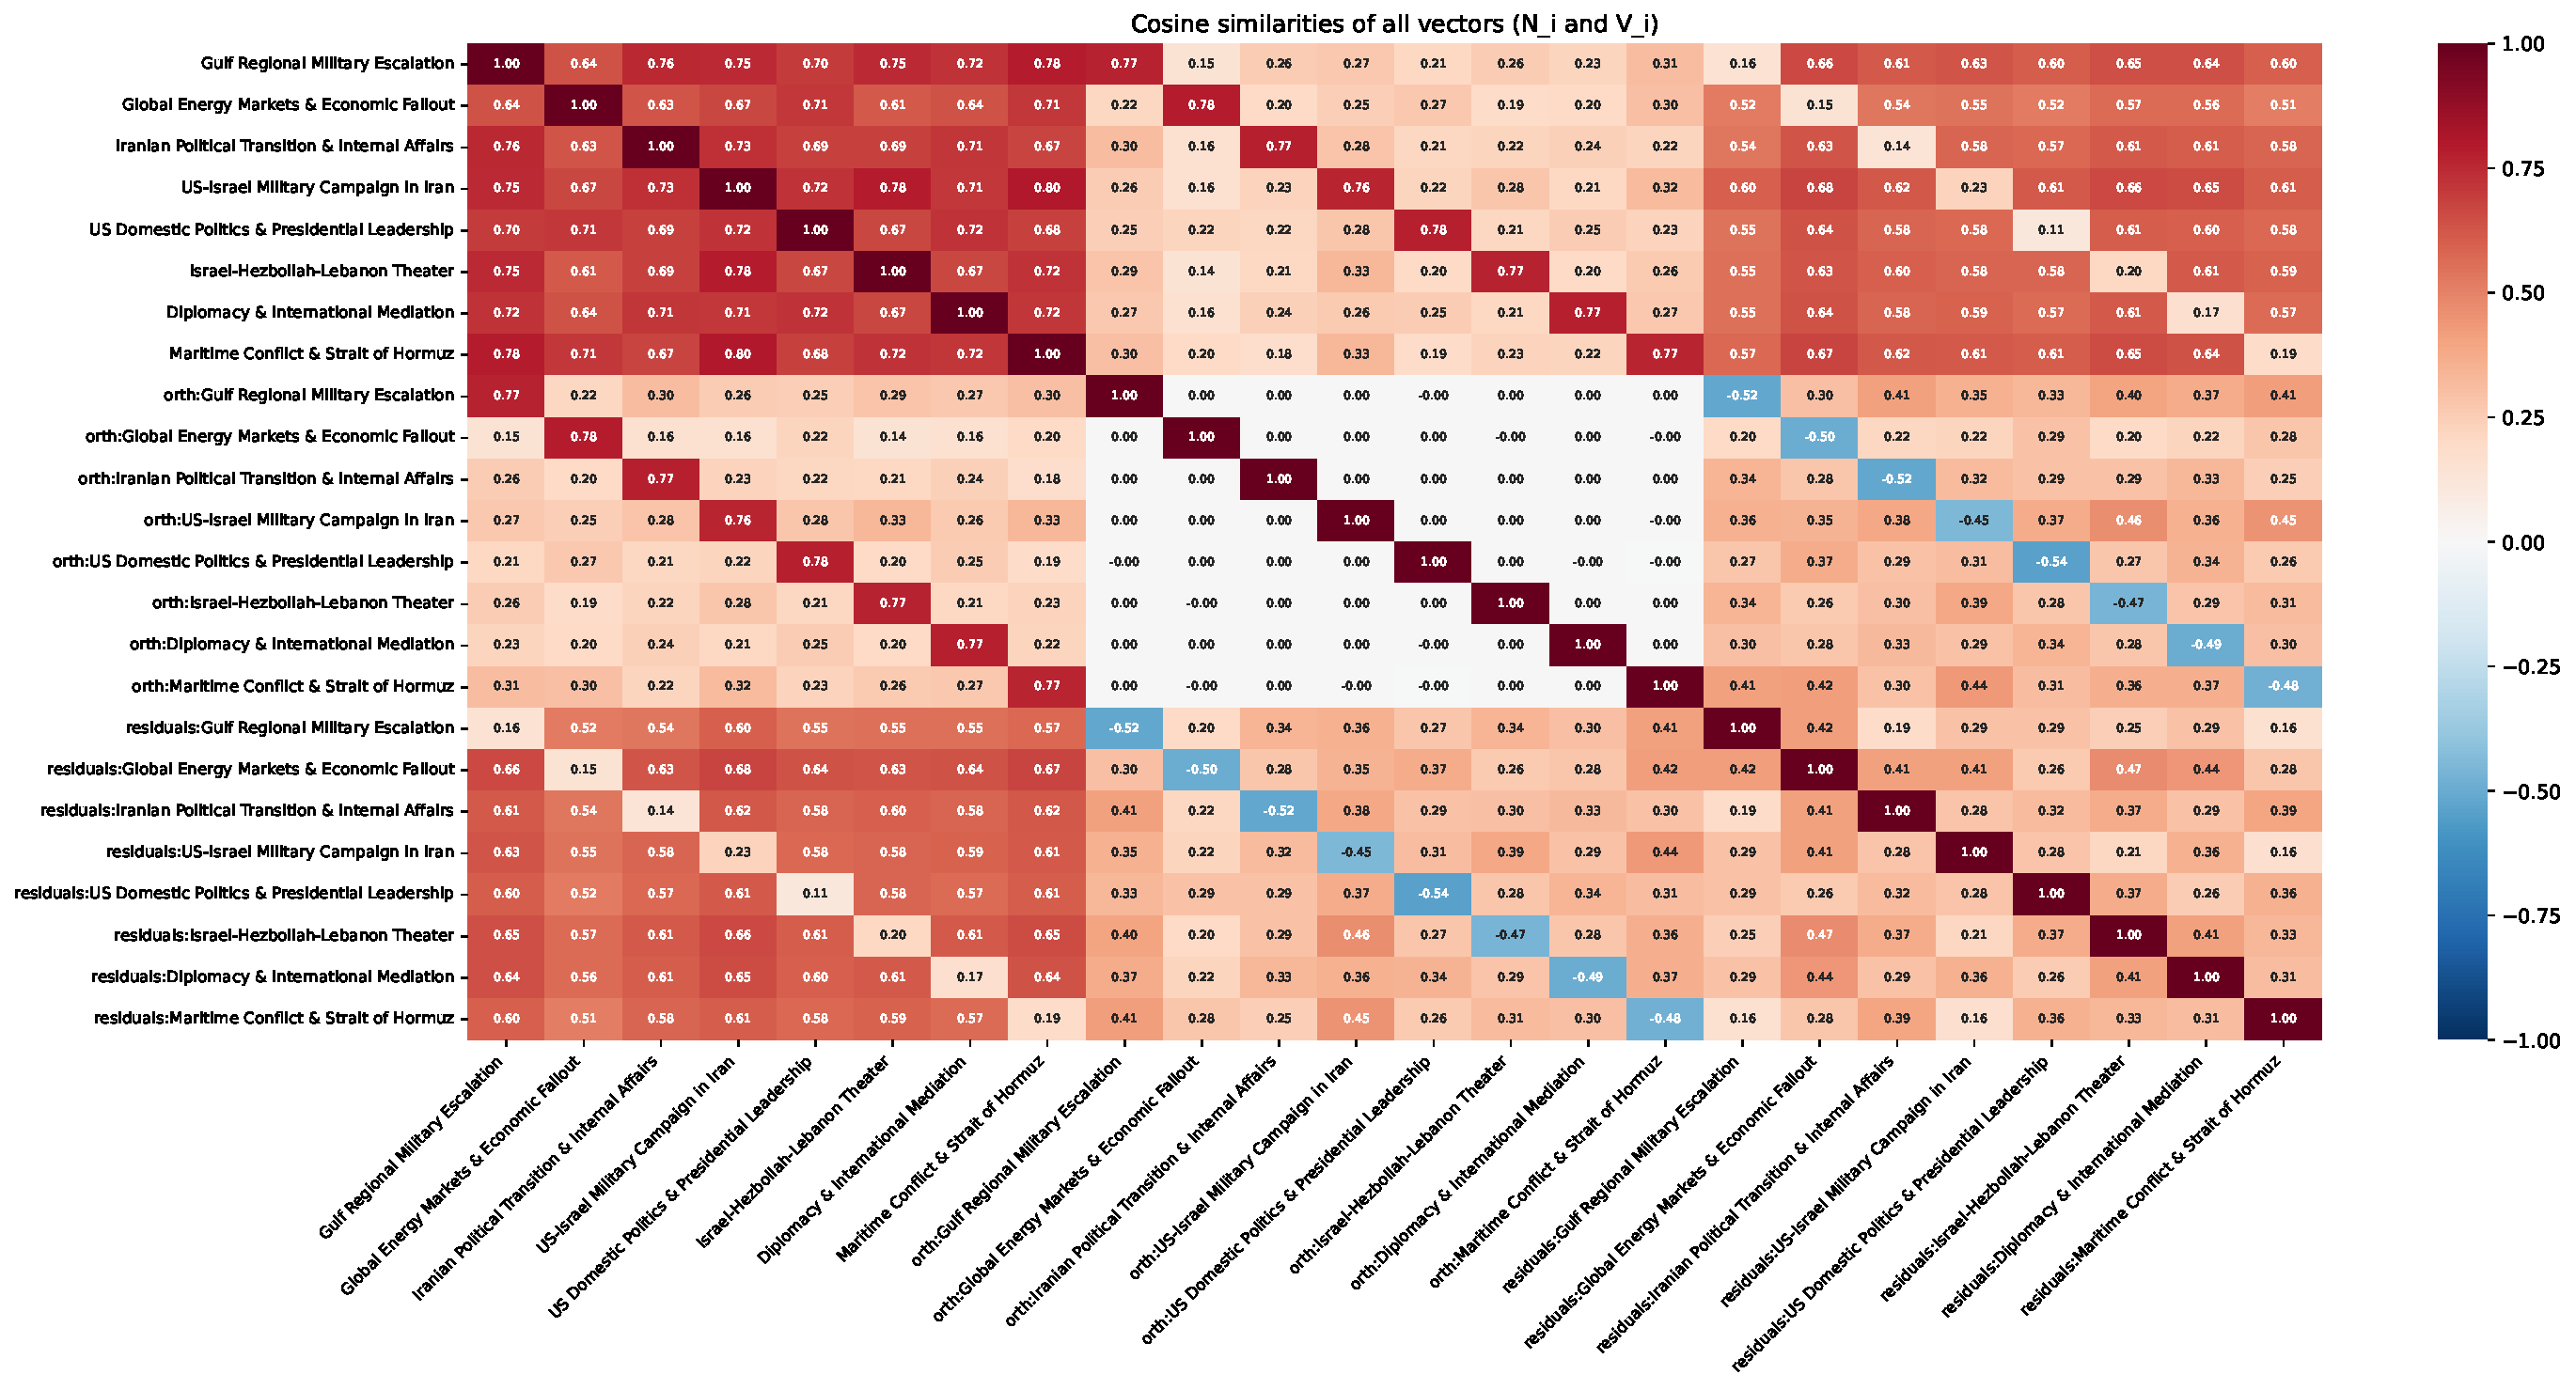
\includegraphics[width=\linewidth]{cosine_similarities_avg.pdf}\\
      {\scriptsize Cosine similarity: originals (top-left), orthogonal (middle), residuals (bottom-right).}
    \end{column}
  \end{columns}
\end{frame}

\begin{frame}
  \frametitle{The Optimization Problem on the Stiefel Manifold}

  Find $V \in \text{St}(K,d) = \{V \in \R^{K\times d}: VV^\top = I_K\}$, as
  close as possible to $N$, by solving a worst-case alignment problem:
  \[
  \max_{V \in \text{St}(K,d)} \ \min_{i=1,\dots,K} \ \langle N_i, V_i\rangle
  \]
  \begin{itemize}
    \item No single narrative is sacrificed to improve the others.
    \item Smoothed via a soft-min surrogate (temperature $\tau=0.05$):
    \[
    \text{softmin}_\tau(x_1,\dots,x_K) = -\tau \log \sum_{i=1}^K \exp\left(-\frac{x_i}{\tau}\right)
    \]
    \item Minimized with \polbf{Riemannian conjugate gradient} (pymanopt),
      initialized by Gram--Schmidt on $N$.
    \item Fast: 24--40 iterations, a few seconds.
  \end{itemize}

  \vspace{.5em}
  \begin{squaredblock}{Three comparable objects per cluster $i$}
  \small
  \polbf{Prototype} $N_i$ (signal + shared noise) $\quad\to\quad$
  \polbf{Pure narrative} $V_i$ (mutually orthogonal by construction)
  $\quad\to\quad$ \polbf{Residual} $R_i = \dfrac{N_i - V_i}{\lVert N_i - V_i\rVert}$ (the removed background noise)
  \end{squaredblock}
\end{frame}

\begin{frame}
  \frametitle{Worked Example: From Prototype to Pure Narrative (Maritime)}

  \begin{itemize}
    \item $N_{\text{Maritime}}$ has cosine similarity $\approx 0.78$ with
      $N_{\text{US-Israel Campaign}}$ and $\approx 0.71$ with
      $N_{\text{Diplomacy}}$ -- shared ``military operations'' /
      ``negotiation'' vocabulary.
    \item After optimization, $V_{\text{Maritime}}$ has, \polbf{by
      construction}, cosine similarity $\approx 0.00$ with every other pure
      narrative, while retaining alignment $\approx 0.77$ with its own
      original direction $N_{\text{Maritime}}$: still recognizably
      ``maritime conflict'', just stripped of what it shared with the rest.
    \item The residual $R_{\text{Maritime}}$ instead correlates
      \polbf{positively} with the other clusters' prototypes ($0.51$--$0.67$)
      and \polbf{negatively} with its own pure narrative ($-0.48$): exactly
      the shared, non-discriminative component removed by orthogonalization.
  \end{itemize}
\end{frame}

% =========================================================================
\section{Stage 4: Scoring Under Three Representations}
% =========================================================================

\begin{frame}
  \frametitle{Three Similarity Matrices per Snippet}

  Every snippet $s_t$ carries a K-Means label $c(t)$ from Stage 1 (obtained
  \emph{before} orthogonalization existed). It is scored against all 8
  prototypes under each representation:
  \[
  S^{\text{orig}}_{t,i} = \mathbf{e}_t^\top N_i, \qquad
  S^{\text{orth}}_{t,i} = \mathbf{e}_t^\top V_i, \qquad
  S^{\text{res}}_{t,i} = \mathbf{e}_t^\top R_i
  \]

  \begin{squaredblock}{Worked example -- one Maritime snippet}
  \footnotesize
  \begin{tabular}{lccc}
    \toprule
    \bf Prototype ($j$) & $S^{\text{orig}}$ & $S^{\text{orth}}$ & $S^{\text{res}}$ \\
    \midrule
    Maritime Conflict (own cluster) & $\sim 0.80$ & $\sim 0.52$ & $\sim 0.30$ \\
    US-Israel Military Campaign & $\sim 0.75$ & $\sim 0.28$ & $\sim 0.55$ \\
    Diplomacy \& Mediation & $\sim 0.70$ & $\sim 0.22$ & $\sim 0.50$ \\
    \bottomrule
  \end{tabular}
  \end{squaredblock}

  \vspace{.5em}
  \polbf{Under original:} own theme wins by a narrow margin (crowded space).
  \polbf{Under orthogonal:} the margin widens sharply once shared signal is
  projected out -- unambiguously closest to its purified theme.
\end{frame}

% =========================================================================
\section{Stage 5: Ex Post Validation}
% =========================================================================

\begin{frame}
  \frametitle{Does Orthogonalization Improve Discrimination?}

  \centering
  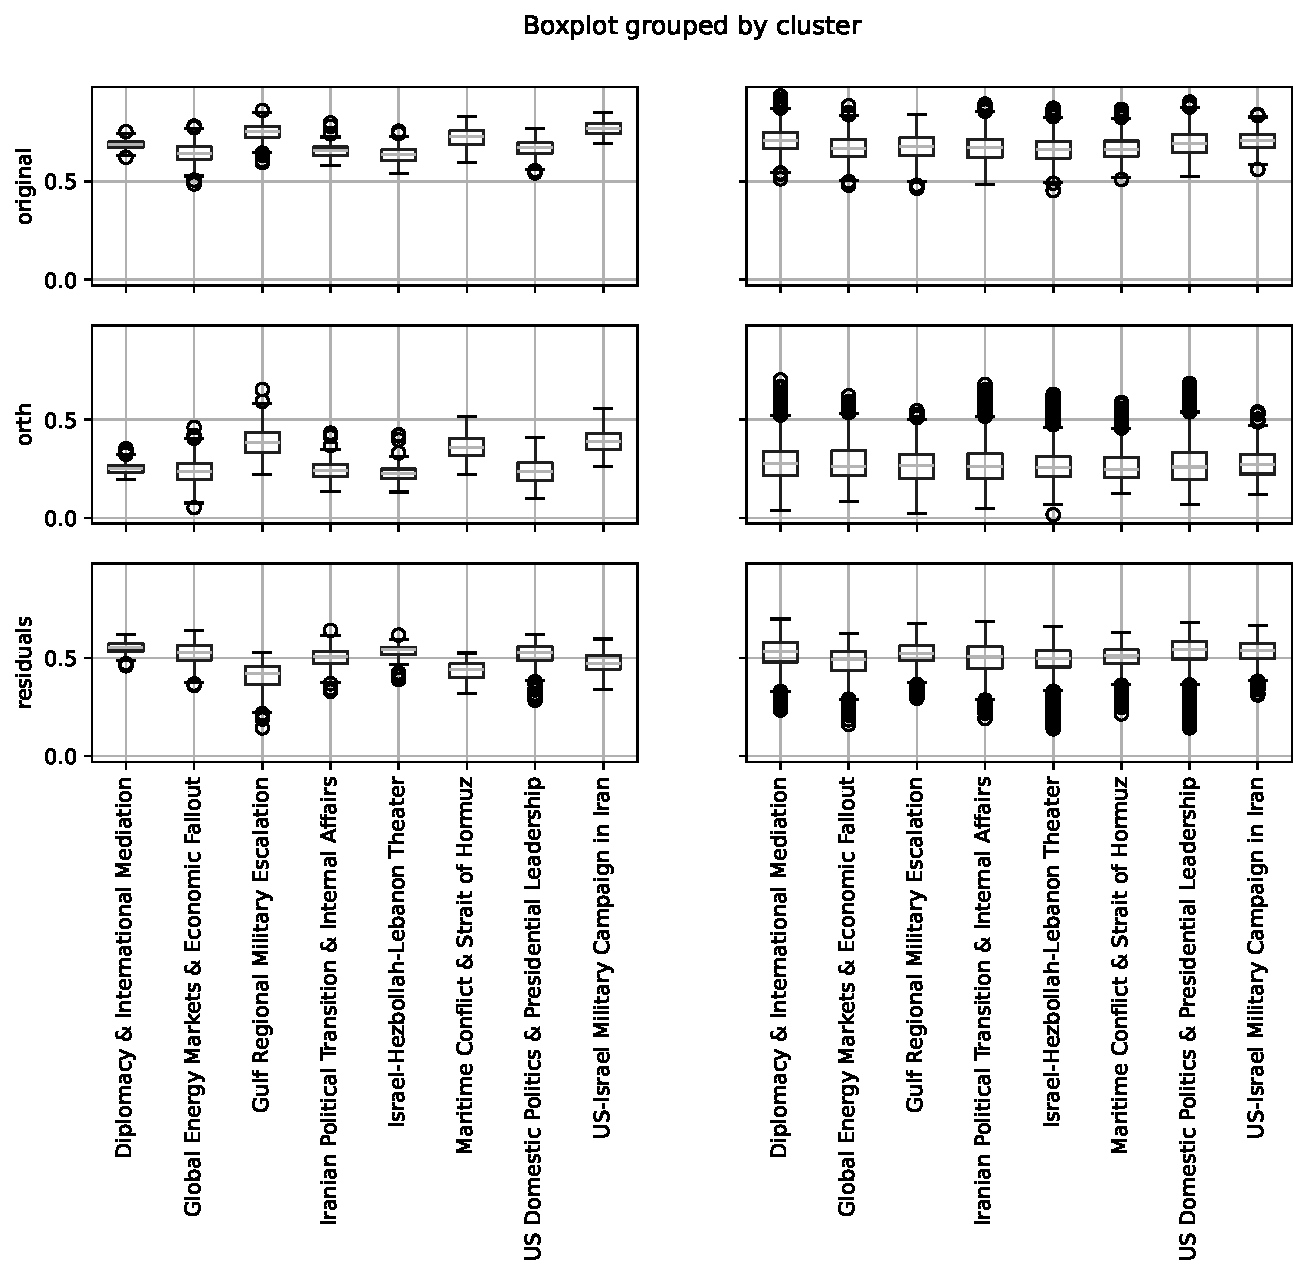
\includegraphics[width=.72\linewidth]{compare_cosine_orth.pdf}\\
  {\scriptsize In-cluster (left) vs. out-of-cluster (right) similarity, by
  theme, under original / orth / residual representations. The gap is small
  for ``original'' and ``residuals'', much larger for ``orth''.}
\end{frame}

\begin{frame}
  \frametitle{Standardized Separation, Theme by Theme}

  \centering
  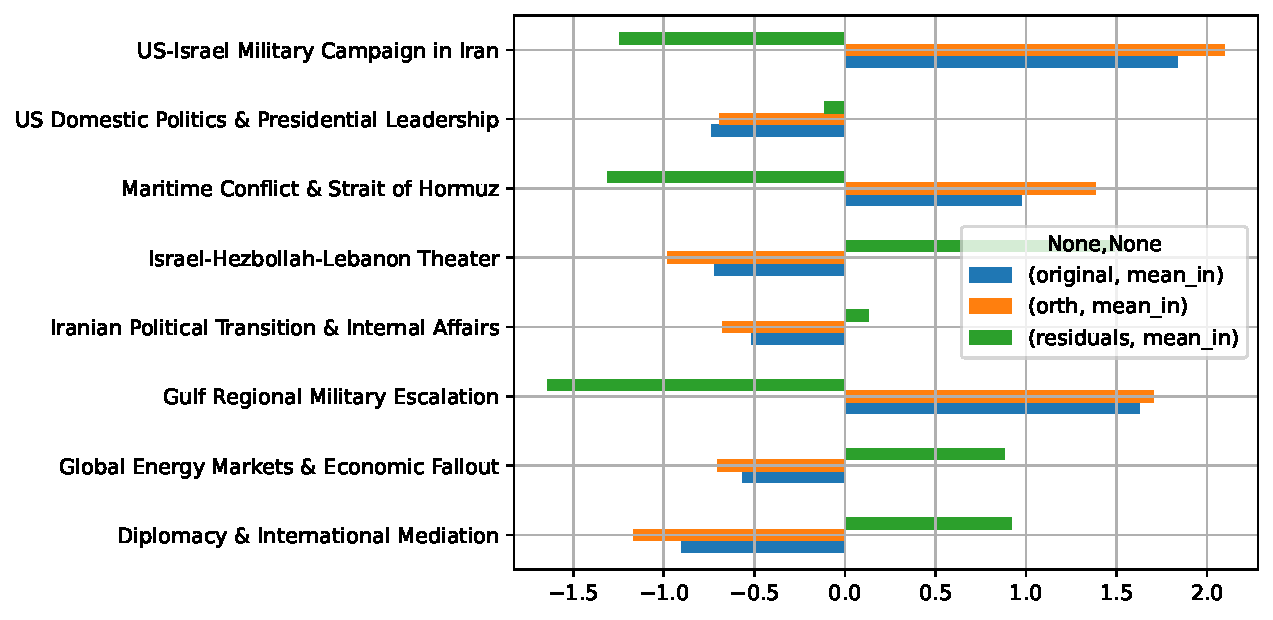
\includegraphics[width=.72\linewidth]{compare_cosine_mean.pdf}\\
  {\scriptsize $(\bar S_{\text{in}} - \bar S_{\text{out}})/\sigma_{\text{in}}$
  for each theme. Orange (orth) $>$ blue (original) for \polbf{every single
  theme}; green (residuals) is uniformly negative.}

  \vspace{.5em}
  \small
  \polbf{Maritime Conflict}: largest gain of all themes --
  $\approx 4.3\,\sigma$ (orth) vs. $\approx 3.5\,\sigma$ (original) -- a
  technical vocabulary (``Strait of Hormuz'', ``tanker'', ``blockade'')
  survives orthogonalization essentially intact.
\end{frame}

\begin{frame}
  \frametitle{Take-Away}

  Across all eight themes, the \polbf{pure-narrative} representation
  \polbf{matches or exceeds} the raw prototype's discriminative power,
  while the \polbf{residual} representation is \polbf{uniformly
  non-discriminative}.

  \vspace{.5em}
  Since pure narratives come from only 3 hand-picked sentences per cluster
  and an unsupervised geometric constraint (orthonormality) -- \emph{not}
  from the K-Means labels -- and since K-Means itself ran on the untouched
  embedding space, this is an \polbf{unsupervised, label-free
  corroboration} that:
  \begin{enumerate}
    \item the 8 K-Means clusters correspond to \polbf{genuinely separable}
      narrative axes;
    \item Stiefel orthogonalization recovers \polbf{additional, meaningful
      discriminative signal} masked by shared background noise;
    \item tracking a document's (or a day's) similarity to a \polbf{pure
      narrative over time} is a meaningful way to monitor exposure to that
      narrative, largely free of confounding drift in generic war-reporting
      language.
  \end{enumerate}
\end{frame}

% THANK YOU
{\usebackgroundtemplate{%
    \IfFileExists{polytechnique_vg_small.jpg}{\includegraphics[width=\paperwidth,height=\paperheight]{polytechnique_vg_small.jpg}}{}} 
  \begin{frame}[label=conclusion, standout]{Thank you for your attention}
    \setcounter{tocdepth}{2}
    \begin{center}
      \rule{0pt}{6em}
      \textcolor{white}{\tt charles-albert.lehalle@polytechnique.edu}
    \end{center}
  \end{frame}
  \usebackgroundtemplate{}
  \setcounter{tocdepth}{2}

\appendix

\begin{frame}[allowframebreaks]
  \frametitle{Appendix: The Eight Clusters, in Detail}
  \footnotesize
  \begin{description}[leftmargin=0cm]
    \item[Cluster 0 -- Gulf Regional Military Escalation ($n=209$)] Direct
      attacks, drone/missile interceptions, evacuations across secondary
      Gulf states (Saudi Arabia, Kuwait, UAE, Bahrain, Qatar, Iraq, Yemen).
    \item[Cluster 1 -- Global Energy Markets \& Economic Fallout ($n=81$)]
      Oil-price surges, market volatility, SPR releases and other economic
      consequences of the war.
    \item[Cluster 2 -- Iranian Political Transition \& Internal Affairs
      ($n=110$)] Internal governance, death of Supreme Leader Khamenei,
      succession, domestic repression.
    \item[Cluster 3 -- US-Israel Military Campaign in Iran ($n=246$)]
      Direct kinetic operations -- airstrikes, missile exchanges, naval
      engagements, CENTCOM updates.
    \item[Cluster 4 -- US Domestic Politics \& Presidential Leadership
      ($n=306$)] White House rhetoric, press briefings, congressional
      oversight debates.
    \item[Cluster 5 -- Israel-Hezbollah-Lebanon Theater ($n=170$)] Parallel
      Israel--Hezbollah/Lebanon front: rocket/airstrike exchanges, fragile
      ceasefires.
    \item[Cluster 6 -- Diplomacy \& International Mediation ($n=235$)]
      Diplomatic backchannels (Qatar, Pakistan, Oman), ceasefire/peace
      frameworks.
    \item[Cluster 7 -- Maritime Conflict \& Strait of Hormuz ($n=215$)]
      Shipping disruption, naval blockades, tanker attacks, transit through
      the Strait of Hormuz.
  \end{description}
\end{frame}

\end{document}
